\documentclass[UTF8]{ctexart}


\usepackage{tikz,mathpazo}
\usetikzlibrary{shapes.geometric, arrows}
\usetikzlibrary{calc}


\usepackage{listings}
%插入代码的配置
\definecolor{CPPLight}  {HTML} {686868}
\definecolor{CPPSteel}  {HTML} {888888}
\definecolor{CPPDark}   {HTML} {262626}
\definecolor{CPPBlue}   {HTML} {4172A3}
\definecolor{CPPGreen}  {HTML} {487818}
\definecolor{CPPBrown}  {HTML} {A07040}
\definecolor{CPPRed}    {HTML} {AD4D3A}
\definecolor{CPPViolet} {HTML} {7040A0}
\definecolor{CPPGray}  {HTML} {B8B8B8}
\lstset{
	language=c,                                     % 设置语言
    columns=fixed,
    breaklines = true,
    basicstyle=\small ,
    numbers=left,                                        % 在左侧显示行号
    %frame=none,                                          % 不显示背景边框
    backgroundcolor=\color[RGB]{245,245,244},            % 设定背景颜色
    keywordstyle=\color[RGB]{40,40,255},                 % 设定关键字颜色
    numberstyle=\tiny\color{darkgray},           % 设定行号格式
    %commentstyle=\it\color[RGB]{0,96,96},                % 设置代码注释的格式
    stringstyle=\rmfamily\slshape\color[RGB]{128,0,0},   % 设置字符串格式
    showstringspaces=false,                              % 不显示字符串中的空格
    %morekeywords={True,alignas,continute,friend,register,true,alignof,decltype,goto,
    %reinterpret_cast,try,asm,defult,if,return,typedef,auto,delete,inline,short,
    %typeid,bool,do,int,signed,typename,break,double,long,sizeof,union,case,
    %dynamic_cast,mutable,static,unsigned,catch,else,namespace,static_assert,using,
    %char,enum,new,static_cast,virtual,char16_t,char32_t,explict,noexcept,struct,
    %void,export,nullptr,switch,volatile,class,extern,operator,template,wchar_t,
    %const,false,private,this,while,constexpr,float,protected,thread_local,
    %const_cast,for,public,throw,std,rand},
    emph={access,and,break,class,continue,def,del,elif ,else,%
	except,exec,finally,for,from,global,if,import,in,i s,%
	lambda,not,or,pass,print,raise,return,try,while},
    emphstyle=\color{CPPViolet},
    emph={[2]True, False, None, self},
	emphstyle=[2]\color{green},
	emph={[3]from, import, as},
	emphstyle=[3]\color{blue},
	upquote=true,
	morecomment=[s]{"""}{"""},
	commentstyle=\color{orange}\slshape,
	emph={[4]1, 2, 3, 4, 5, 6, 7, 8, 9, 0},
	emphstyle=[4]\color{red},
	emph={[5]numpy, np, plt},
	emphstyle=[5]\color{red},
	literate=*{:}{{\textcolor{blue}:}}{1}%
	{=}{{\textcolor{blue}=}}{1}%
	{-}{{\textcolor{blue}-}}{1}%
	{+}{{\textcolor{blue}+}}{1}%
	{*}{{\textcolor{blue}*}}{1}%
	{!}{{\textcolor{blue}!}}{1}%
	{(}{{\textcolor{blue}(}}{1}%
	{)}{{\textcolor{blue})}}{1}%
	{[}{{\textcolor{blue}[}}{1}%
	{]}{{\textcolor{blue}]}}{1}%
	{<}{{\textcolor{blue}<}}{1}%
	{>}{{\textcolor{blue}>}}{1},%
	framexleftmargin=0.1mm, framextopmargin=0.1mm, frame=shadowbox, rulesepcolor=\color{black},
 escapeinside=``,
}



\usepackage{geometry}
\geometry{left=2cm, right=2cm, top=2cm, bottom=2cm}
\usepackage{appendix}
\usepackage{underscore}
%得到引用的标题内容
\usepackage{nameref}

%添加首行缩进,两个字符
\usepackage{indentfirst}
\setlength{\parindent}{2em}

%多行公式一个编号
\usepackage{amsmath}

%文献引用,标准类型为plain
%\usepackage[hyperref=true,backend=biber,sorting=none,backref=true]{biblatex}
%\addbibresource{ref.bib}
\bibliographystyle{plain}
\usepackage{cite}

\pagestyle{plain}


\usepackage{graphicx}

%超链接
\usepackage[linkcolor=yellow,citecolor=red,backref=page]{hyperref}
\hypersetup{
bookmarks=true,
colorlinks=true,
linkcolor=black
}

%引入了一些改进的数学环境,如align
\usepackage{amsmath}

\title{课题五:点阵广告牌的设计}
\author{姓名:寇一笑 \protect\newline
\and 学号:18020024016 \\
\and 专业:电子信息科学与技术}


\begin{document}
	\maketitle
	\renewcommand{\contentsname}{Contents}
	\tableofcontents
	\newpage
	
	\hypersetup{
	bookmarks=true,
	colorlinks=true,
	linkcolor=red,
	urlcolor=blue
	}
\begin{abstract}
因为软件经常崩溃以及在一个文件加载多片单片机会出现无法响应问题,作业分为了$billboard$、$background music$、$eating snake$三个文件夹提交。下面的报告就是按照三个文件夹进行描述的。大致对应基础中级高级功能,不过基础和中级有一部分是混合的。
\end{abstract}

	\section{billboard}
\subsection{任务分析及其思路}
$billboard$文件\footnote{设计参考了https://blog.csdn.net/qq_41639829/article/details/82726377?tdsourcetag=s_pcqq_aiomsg}的任务是要利用51单片机和点阵滚动显示字符,并且滚动的方向可以通过外部输入设备进行调整。\par
对于这样一个任务我们首先需要明确点阵显示图形的原理。所谓显示图形,实质上就是把特定位置的LED灯点亮。我们的做法是先选中一行(列),即向对应的管脚输出高电平或低电平,取决于该点阵是行共阳还是行共阴;然后再选中对应的列,同样是向对应的管脚输出相应电平。区别是这样做时一般只会选中一行,但可能选中多列。这样做也是为了显示需要。由于结构本身的限制,我们不可能同时对多行多列进行操作。所以只能把一个图形拆成一行一行来扫描。而由于人眼有视觉暂留效应,只要扫描的速度够快,我们看到就是一副完整的图像。\par
当然,也可以先选中列再选中行,道理是一样的。这里我们两种方法都要用到。\par
以上说的是静态显示,而滚动显示就是当扫完最后一行后回到第一行时,对应列需要点亮的是上一轮的第二行的位置。同样,第二行要点亮上一轮第三行的位置,第三行要点亮上一轮第四行的位置……最后一行要点亮上一轮最后一行的下一行需要显示的位置。相当于整个图形向上移动了一格。\par
这样我们就完成了从上往下的滚动显示,从下往上其实就是刚好把上述过程反过来:第二行点亮上一轮第一行的位置,第三行点亮上一轮第二行的位置……\par
而左右滚动的原理也是类似的。只不过此时我们是先选中一列,再选中对应的若干行,一列一列进行扫描。相当于把上下滚动中的行列地位交换了。
\subsection{硬件设计分析}
\subsubsection{74HC595}
此次课程设计中我们用到的芯片有51单片机,LED点阵以及74HC595串行输入、并行输出的位移缓冲器\par
51单片机和点阵的作用自不必说。这里需要用到74HC595的原因是一个点阵需要单片机提供32个接口去分别控制它的16行和16列,但显然51单片机做不到这一点。所以此时我们需要用74HC595来对接口进行扩展。\par
74HC595可以通过DS引脚接受单片机输入的串行数据,然后把得到的8位串行数据转成并行数据再输出。这样单片机只需要提供一个引脚就可以输出8位数据,相当于把一个引脚当八个来用。\par
同时这里我们对74HC595进行了级联,两个一组能够同时输出16位数据。这样我们就可以只用两个单片机接口来分别控制点阵的行和列了。\par
当然,这里对每一组74HC595还需要两个时钟信号来对DS引脚上的信号进行接收和移位处理。所以总共要用到六个接口。
\subsubsection{中断}
 51单片机的外部中断电路比较简单,只需要通过按钮把P3.2和P3.3引脚接地即可。
\subsection{软件设计分析}
\subsubsection{向74HC595输送数据}
这里我们为了简化程序,需要专门写函数来给74HC595输送数据。由于上下滚动和左右滚动在输送数据时稍有不同,所以我们总共写了四个函数,分别用于在上下滚动时向行列送数据和在左右滚动时向行列输送数据。\par
以上下滚动为例,首先我们需要选中一行。这时需要往控制行的那一组74HC595输送一个16位的数,被选中的哪一行对应位是0,其余为1。由于要一位一位地输出,所以我们每次先把要输送的数跟8000H相与,即只保留最高位,把计算的结果输出,然后令待输出的数左移移位,再重复上述过程。\par
需要注意的一点是,在每次输出的过程中,要令控制74HC595移位寄存器时钟和存储寄存器时钟的变量置0、置1,否则数据无法被正确读入。\par
向控制列的那一组74HC595输送数据的函数基本与上面所说的相同。只是此时向列输送的是字码,而字码我们在计算时是以8位二进制数的形式存放的。所以在输送前要与80H相与。
同时在调用这个函数时也要注意,输出一行的字码要用两次该函数。\par
左右滚动与上下滚动输出数据的过程基本一致,只不过此时向控制行的那组74HC595输出的是字码,所以在该函数中待输出数据应与80H相与;而相应的,向控制列的那组74HC595输出时要与8000H相与。\par
另外在左右滚动时还有一点需要特别注意,选通行时要输出低电平,选通列时要输出高电平,而我们的字码和选通行列的数据都是按上下滚动时计算的,即字码是为列选通而计算的,用于选通的数是按行来计算的。前面我们说过,左右滚动时行列的地位要颠倒,所以此时对字码和用于选通的数都要先按位取反再作为函数参数调用。\par
\subsubsection{滚动显示}
点阵要进行滚动显示就意味着,每一轮向点阵输出的16行字码要整体向后挪一位。所以我们这里定义一个变量,每一轮以这个变量的值为起始,向后输出16行字码。然后再令该变量加2(一行字码用的是两个8位的二进制数存放的,故应加2)。同时为了保证输出完所有字之后能循环回第一个字,当该变量的值要超过字码数组的值时我们把它置0。而如果要反向滚动,则每次令该变量减2即可。相应的,为了使反向的滚动也能够循环,我们在该变量小于0时把它置为数组的长度减一(原因仍然是两个字码为一行)。\par
\subsubsection{中断函数}
电路设计中我们用到了两个中断源,分别控制上下滚动的方向和左右滚动的方向。所以这里我们也要用两个变量hang_flag和lie_flag来表示上下滚动和左右滚动的方向。这里我们用1来表示从上往下或从左往右,用-1表示从下往上或从右往左。所以在中断函数中我们要做的其实就是令相应的标志乘上-1即可。同时还要注意的是,在调用控制行方向的中断时,要令lie_flag为0;在调用控制列方向的中断时,要令hang_flag为0。
\subsubsection{软件设计流程图}
\begin{figure}[ht]
	\centering
	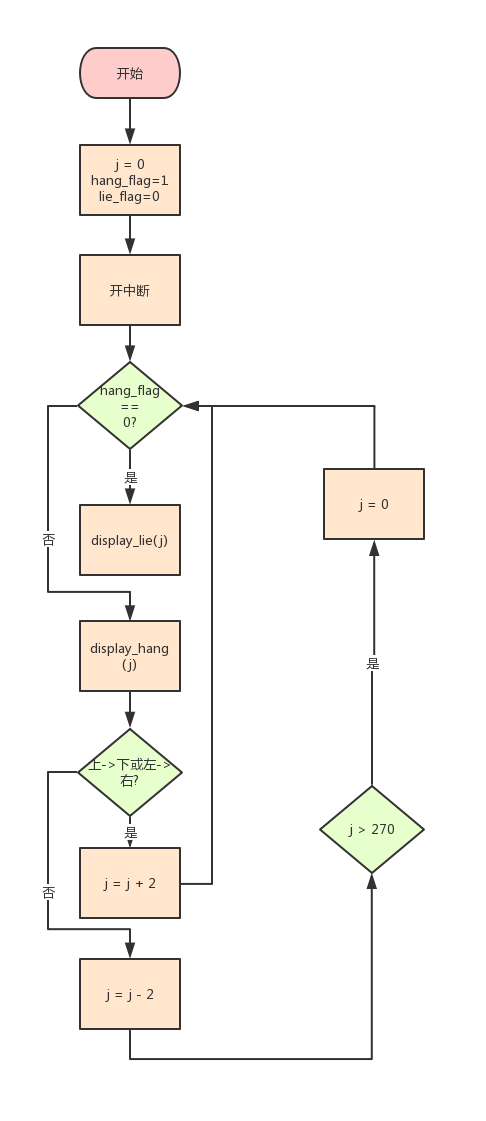
\includegraphics[scale=0.3]{1.png}
\end{figure}
\subsection{记录}
在滚动显示中,这里有一个特别容易被忽略的地方,就是原作者在定义这个变量时用的是unsigned int类型,所以它在减到0后不会出现负数的情况,而是会溢出。所以这里我们不能直接判断它是否为负数。但是仔细考虑下我们会发现,溢出后的值肯定是大于数组长度的,所以在正向滚动时用的那个判断条件这里仍可以用,只是把置0改为置数组长度减一。\par
在中断函数中,外部中断1对应的中断号是2。之前想当然地以为是1,结果左右滚动怎么都出不来,在这上面卡了很久。\par
关于字模我一开始尝试了GBK汉字的十六进制转换,但是生成的太短,后来受到一篇显示汉字实验,自己制作字模,但是仍然编译不成功,最后在github找到了PCtoLCD2002字模软件,但是生成的还是乱码,这里要注意阴码和阳码的区别。
    \section{background music}
    \subsection{概述}
    $background music$主要实现的是通过三个按键来实现播放三首不同的音乐,同时另外设置一个按键实现停止音乐。\par
    根据资料查找我知道,一般单片机演奏音乐基本都是单音频率,它不包含相应幅度的谐波频率,不能像电子琴一样奏出多种银色的声音。对于音乐中的每一个音调,或者说我们常说的“音高”,我们只要知道其基本音调的频率,然后通过单片机的定时器定时中断,将单片机上对应蜂鸣器的I/O口来回取反,或者说来回清零、置位,从而让蜂鸣器发出声音。为了让单片机发出不同的频率的声音,我们只要将定时器置不同的定时值即可实现。那么如何确定一个频率所对定的定时器的定时值呢?以标准音高A为例:\par
    A的频率为440Hz,其对应的周期为:
    \begin{center}
    $T=1/f=1/440=2272\mu s$
    \end{center}
    那么单片机上的对应蜂鸣器的I/O口来回取反的时间应为:
    \begin{center}
    $t=T/2=2272/2=1136\mu s$
    \end{center}
    这个时间t也就是单片机上定时器应有的中断触发时间。一般情况下,单片机奏乐时,其定时器为工作方式1,它以振荡器的之二分频为计时脉冲。设振荡器频率为$f_0$,则定时器的予置初值由下式来确定:
    \begin{center}
      $t=12*(T_{ALL}-T_{HL})/f_0$
    \end{center}
    式中$T_{ALL}=2^{16}=65536$,$T_{HL}$为定时器待确定的计数初值。因此定时器的高低计数器的初值为:
    \begin{center}
      $TH=T_{HL}/256=(T_{ALL}-t*f_{0}/12)/256$\\
      $TL=T_{HL}/256=(T_{ALL}-t*f_{0}/12)/256$
    \end{center}
    将$t=1136\mu s$代入上式即可赋予计数器初值。
    \subsection{硬件设计}
    \subsubsection{AT89C51}
    设计里面使用到了AT89C51,它与AT89C52相比功能略有欠缺,比如RAM空间、内部FLASH会变小,中断源数量也会变少,但是其他功能和用法基本与C52相近。
    \subsubsection{74HC11}
    74HC11是三输入端三与门,主要负责将选的歌的按钮的电平读到$\overline{\mathrm{INT0}}$引脚
    \subsubsection{三极管与喇叭}
    三极管使用共集接法,此处不涉及放大电信号,那么三极管就当做开关用。如上所述,通过单片机的定时器定时中断,将单片机上对应蜂鸣器的I/O口来回取反,或者说来回清零、置位,从而让蜂鸣器发出声音
    \subsection{软件设计}
    \subsubsection{延时函数}
    延时函数用在了两个地方,第一处用在了音长延时,使得声音能够连续。第二处用在了开始时延时,使得声音播放不那么突兀。
    \subsubsection{音阶播放函数}
    我们首先根据概述中的方法,将不同的音高转化为计数器初值。并且将不同的歌曲的所有音调的计数器初值存到不同的数组当中,并且将$0xff$看成是结束的标志。当函数传入数组的计数器初值时,如果没有读到按钮中断或者结束符0xff,那么就取高4位音阶得到$T_{H}$和$T_{L}$,然后取低4位进行延时,并且对简谱音调计数 。
    \subsubsection{中断}
    分情况讨论。当不读入0xff时候,那么就继续播放。当收到某个按钮中断的时候,首先判断是从哪个端口读入的,然后  keyValue存储相应的键值,并播放对应的音乐
    \subsubsection{流程图}
    \begin{figure}[ht]
	\centering
	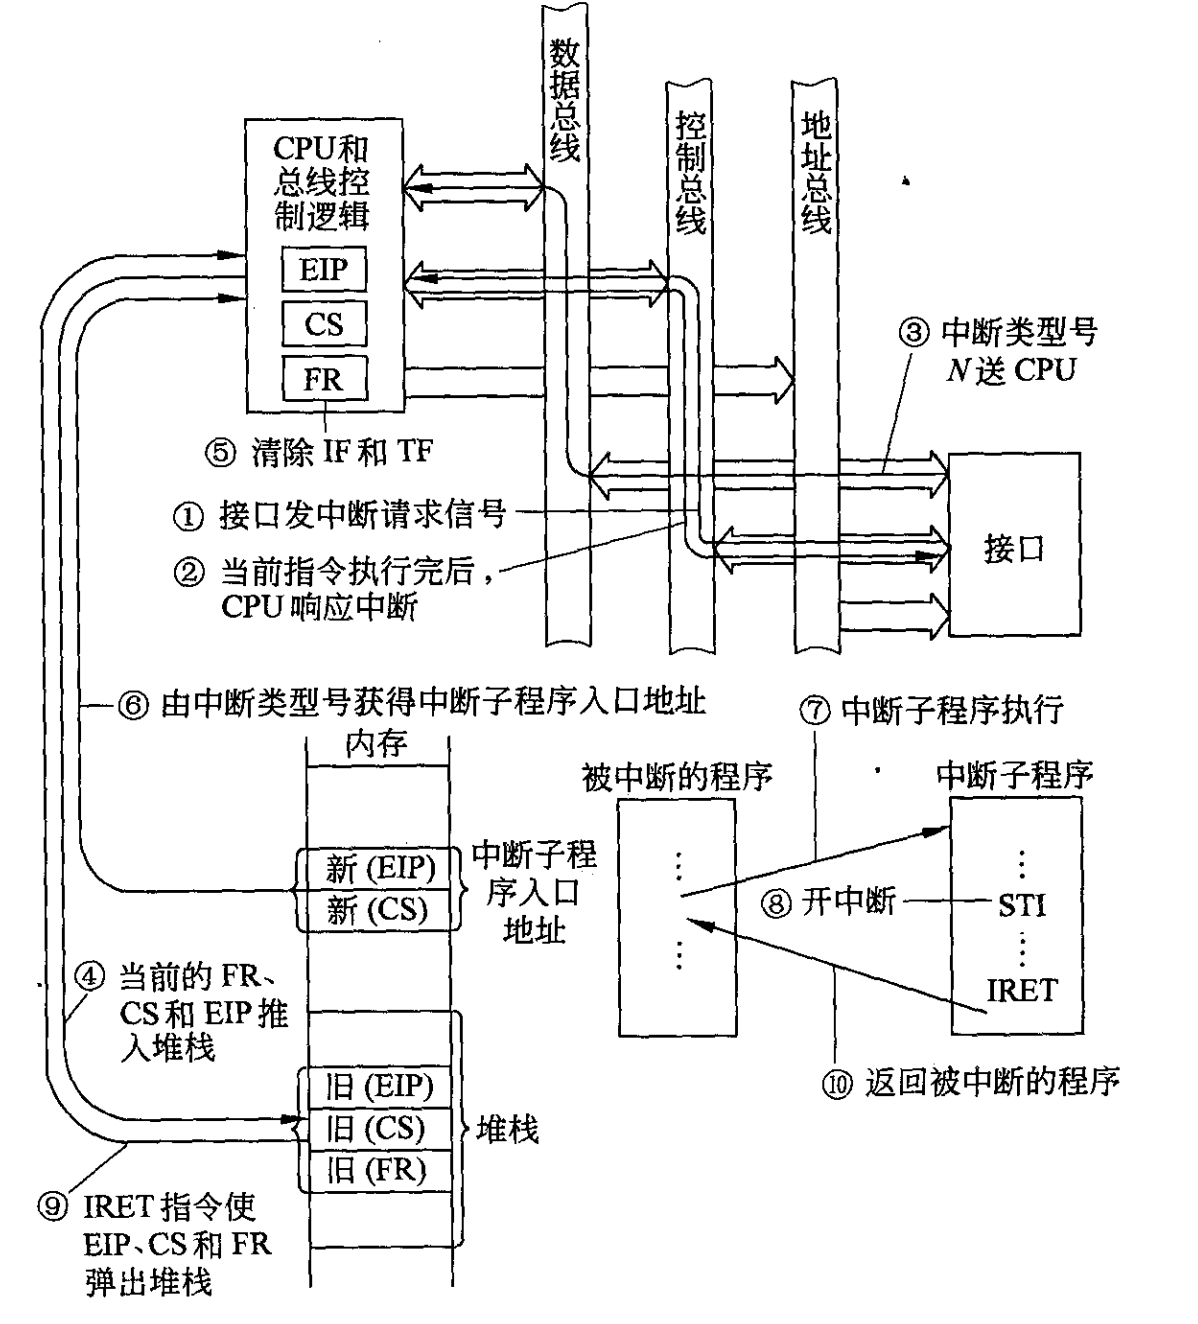
\includegraphics[scale=0.6]{2.png}
\end{figure}
    \subsection{记录}
    关于如何让喇叭发出声音,用到了fx_buzzer=~fx_buzzer,这个指令,百思不得其解,后来了解到将单片机上对应蜂鸣器的I/O口来回取反,或者说来回清零、置位,从而让蜂鸣器发出声音
    \section{eating snake}
    \subsection{概述}
    本设计为一款贪吃蛇游戏,显示器采用8*8点阵,主控制器采用51单片机,并通过按键实现对游戏的操作。\par
    贪吃蛇游戏算法的实现,即如何通过液晶屏显示蛇的移动如下。
    \begin{enumerate}
      \item 其实蛇看似移动的过程中,实质只有两个点再变,即蛇头前进方向增加一个点,蛇尾减少一个点。
      \item 知道如何显示蛇的移动后,再一个关键问题就是蛇的转折问题,如何控制蛇尾消失的点沿着蛇的路径。通俗的说就是蛇怎么实现曲折移动,这里就用到了循环队列,每次蛇头前进方向发生变化后,队列增加一个结点,结点中包含蛇头方向变化的位置,以及蛇头转变的方向。
      \item 蛇尾每次移动的过程中都会与队列头指针所储存的位置做一次判断,当蛇尾到达这一位置后,从结点中取出保存的蛇头的移动方向赋给蛇尾,结点出队列即删除这一结点。
      \item 由于队列是头出尾进,所以蛇头先产生的结点,蛇尾会先与其进行判断,并且删除它,即实现了蛇的曲折运动。
    \end{enumerate}

    \subsection{硬件设计}
    \subsubsection{8*8LED矩阵电路}
            \begin{figure}[ht]
	\centering
	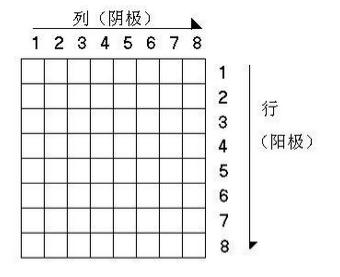
\includegraphics[scale=0.6]{3.png}
\end{figure}
    从图中可以看出,8X8点阵共需要64个发光二极管组成,且每个发光二极管是放置在行线和列线的交叉点上,当对应的某一列置1电平,某一行置0电平,则相应的二极管就亮;要实现显示图形或字体,只需考虑其显示方式。通过编程控制各显示点对应LED阳极和阴极端的电平,就可以有效的控制各显示点的亮灭。
    \subsubsection{按键电路}
    在此设计中设置了五个按键,分别为方向使能、上、下、左、右,方式为当方向使能按键按下后,四个方向的按键动作才有效。
    \subsection{软件设计}
    \subsubsection{用数组表示位置}
    我们定了最大的蛇的长度变量SNAKE为20,以此定义了两个一维数组x[SNAKE+1]、y[SNAKE+1]表示在点阵中的位置。其中一开始用x[0]、y[0]表示果子的x轴和y轴坐标,x[1]、y[1]表示蛇头的x轴和y轴坐标,x[2]、y[2]表示蛇尾的x轴和y轴坐标。以后用x[i]、y[i]表示身体的各个部分的坐标。
    \subsubsection{判断结束}
    当蛇头的坐标X[1]、y[1]超过点阵的范围的时候,判断为与墙面碰撞。当蛇头的坐标X[1]、y[1]等于身体某一部分的坐标x[i]、y[i],判断为与身体碰撞。两种碰撞都直接break。
    \subsubsection{方向处理}
    使用了addx,addy作为对蛇头下一个位置的判定,addx和addy分别可以取1、-1、0,需要注意的是如果蛇往右边走,那么左边方向键是无效的,其他的情况也是一样。如果想往左边走,那么addx=-1,addy=0。
    \subsubsection{判断吃到了果子}
    如果蛇头的坐标加上addx,addy坐标等于果子的坐标,那么执行吃到果子的操作,伸长身体。此时对于数组x[i],y[i],依次执行向后延伸,即身体的原来第二部分变为了现在的第三部分,并且蛇头的坐标为原来蛇头的坐标加上addx,addy坐标。
    \subsubsection{流程图}
                \begin{figure}[ht]
	\centering
	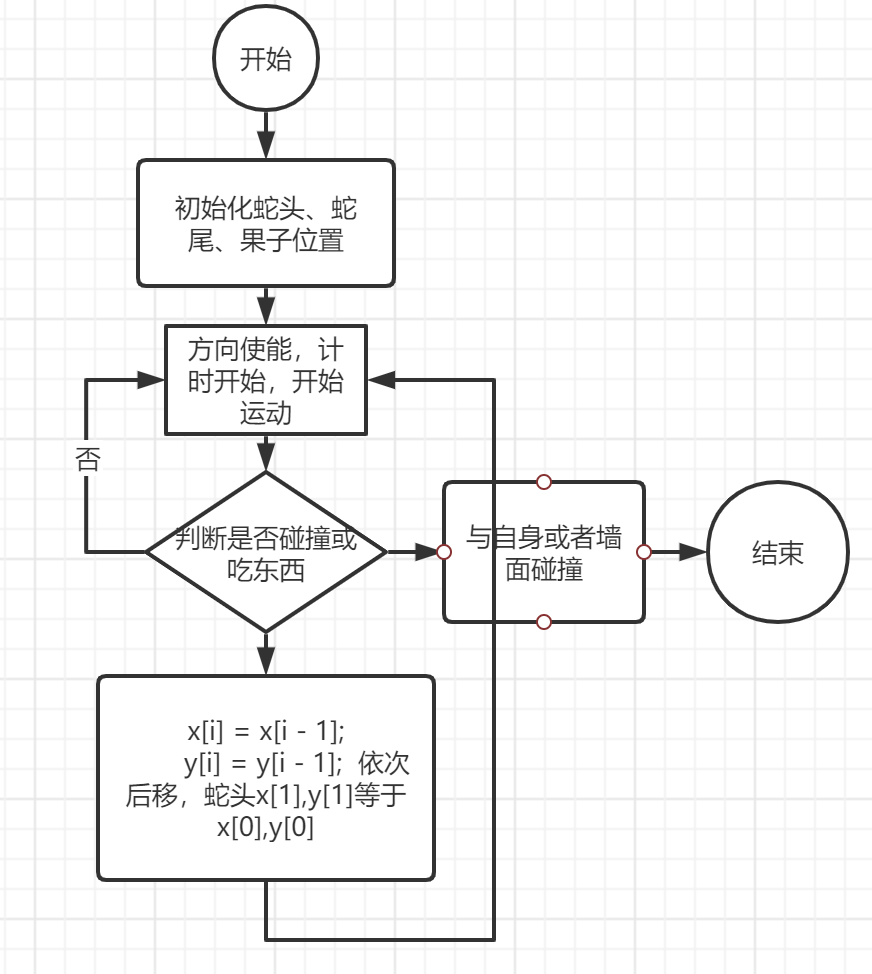
\includegraphics[scale=0.6]{4.png}
\end{figure}
    \subsection{记录}
    这个程序比较难的点在于如何表示蛇每个部分的坐标。之后按照坐标对于不同情况进行讨论就相对比较简单了。
	\section{所有实现的成果}
    三个文件实现的所有成果包括显示不同字符以及动态展示(基础功能第一点,中级功能第二点),用独立按键控制字符正反播放,横向竖向播放(基础功能第二点),贪吃蛇(高级功能),基本实现所有要求。

\appendix
  \renewcommand{\appendixname}{Appendix~\Alph{section}}

  \section{billboard代码}
  \begin{lstlisting}
#include `<reg51.h>`
#include`<intrins.h>`

`/*  数据端接口定义 */`
sbit  LSH = P2^0;     `//列数时钟`
sbit  LDS = P2^1;     `//输入`
sbit  LST = P2^2;     `//列寄存器`

sbit  HSH = P2^3;     `//行数时钟`
sbit  HDS = P2^4;     `//输入`
sbit  HST = P2^5;     `//行寄存器时钟`

int hang_flag=1;
int lie_flag=0;

unsigned int sel[17]={0x7fff,0xbfff,0xdfff,0xefff,0xf7ff,0xfbff,0xfdff,0xfeff,
					0xff7f,0xffbf,0xffdf,0xffef,0xfff7,0xfffb,0xfffd,0xfffe,0xffff};

char code hanzi_hang[272] =
{
0x01,0x00,0x01,0x00,0x01,0x00,0x3F,0xF8,0x21,0x08,0x21,0x08,0x21,0x08,0x3F,0xF8,
0x21,0x08,0x21,0x08,0x21,0x08,0x3F,0xF8,0x21,0x0A,0x01,0x02,0x01,0x02,0x00,0xFE,`//电`
0x00,0x00,
0x00,0x00,0x7F,0xF8,0x00,0x10,0x00,0x20,0x00,0x40,0x01,0x80,0x01,0x00,0xFF,0xFE,
0x01,0x00,0x01,0x00,0x01,0x00,0x01,0x00,0x01,0x00,0x01,0x00,0x05,0x00,0x02,0x00,`//子`
0x00,0x00,
0x01,0x00,0x01,0x00,0x7F,0xFC,0x01,0x00,0x1F,0xF0,0x00,0x00,0x7F,0xFE,0x40,0x02,
0x9F,0xF4,0x00,0x00,0x1F,0xF0,0x10,0x10,0x1F,0xF0,0x08,0x20,0x04,0x40,0xFF,0xFE,`//壹`
0x00,0x00,
0x20,0x80,0x10,0x80,0x00,0x9C,0x47,0xE0,0x20,0x80,0x08,0x84,0x10,0x84,0x60,0x7C,
0x21,0x00,0x01,0x00,0xFF,0xFE,0x05,0x40,0x09,0x20,0x31,0x18,0xC1,0x06,0x01,0x00,`//柒`
0x00,0x00,
0x01,0x00,0x00,0x80,0x3F,0xFE,0x20,0x80,0x2F,0xF8,0x20,0x88,0x3F,0xFE,0x20,0x88,
0x2F,0xF8,0x28,0x80,0x24,0xC4,0x22,0xA8,0x44,0x90,0x48,0x88,0x92,0x86,0x01,0x00,`//康`
0x00,0x00,
};

char code hanzi_lie[272] =
{
0x01,0x00,0x01,0x00,0x01,0x00,0x3F,0xF8,0x21,0x08,0x21,0x08,0x21,0x08,0x3F,0xF8,
0x21,0x08,0x21,0x08,0x21,0x08,0x3F,0xF8,0x21,0x0A,0x01,0x02,0x01,0x02,0x00,0xFE,`//电`
0x00,0x00,
0x00,0x00,0x7F,0xF8,0x00,0x10,0x00,0x20,0x00,0x40,0x01,0x80,0x01,0x00,0xFF,0xFE,
0x01,0x00,0x01,0x00,0x01,0x00,0x01,0x00,0x01,0x00,0x01,0x00,0x05,0x00,0x02,0x00,`//子`
0x00,0x00,
0x01,0x00,0x01,0x00,0x7F,0xFC,0x01,0x00,0x1F,0xF0,0x00,0x00,0x7F,0xFE,0x40,0x02,
0x9F,0xF4,0x00,0x00,0x1F,0xF0,0x10,0x10,0x1F,0xF0,0x08,0x20,0x04,0x40,0xFF,0xFE,`//壹`
0x00,0x00,
0x20,0x80,0x10,0x80,0x00,0x9C,0x47,0xE0,0x20,0x80,0x08,0x84,0x10,0x84,0x60,0x7C,
0x21,0x00,0x01,0x00,0xFF,0xFE,0x05,0x40,0x09,0x20,0x31,0x18,0xC1,0x06,0x01,0x00,`//柒`
0x00,0x00,
0x01,0x00,0x00,0x80,0x3F,0xFE,0x20,0x80,0x2F,0xF8,0x20,0x88,0x3F,0xFE,0x20,0x88,
0x2F,0xF8,0x28,0x80,0x24,0xC4,0x22,0xA8,0x44,0x90,0x48,0x88,0x92,0x86,0x01,0x00,`//康`
0x00,0x00,
};

`// 上下滚动`
void send_data_H_hang(unsigned int dat);  `/*  发送行数据端数据函数  */`
void send_data_L_hang(unsigned int dat);  `/*  发送列选通端数据函数  */`
void display_hang(int a);                 `//每一次显示什么东西`

`// 左右滚动`
void send_data_H_lie(unsigned int dat);  `/*  发送行数据端数据函数  */`
void send_data_L_lie(unsigned int dat); ` /*  发送列选通端数据函数  */`
void display_lie(int a);                ` //每一次显示什么东西`

void delay(unsigned int m);


void main()
{
  unsigned int j=0,num;
  EA = 1;     `//开总中断`
  EX0 = 1;    `//开外部中断0`
  EX1 = 1;
  IT0 = 1;    `//选择电平负跳变触发方式`
  IT1 = 1;
	while(1)
	{
		num=9;
		while(num--)
		{
		    if (lie_flag == 0)
			{
			    display_hang(j);
		    }
			else if(hang_flag == 0)
			{
			    display_lie(j);
			}
			delay(10);

	    }
		if ( (hang_flag==1&&lie_flag==0) || (lie_flag == 1 && hang_flag == 0) )
		{
		    j=j+2;
	    }
		else if ( (hang_flag == -1 && lie_flag == 0) || (lie_flag == -1 && hang_flag == 0) )
		{
		    j = j - 2;
			if(j>270)
			    j=270;
		}
		
		
	}
}
	
void send_data_L_hang(unsigned int dat)
{
    unsigned char i;

    for(i=0;i<8;i++)
    {
        LSH = 0;
        LDS = dat&0x80;       //temp<<=1;
        dat = dat<<1;               //ds = CY;
        LSH = 1;
    }
		LST = 0;
    _nop_();
    _nop_();
    LST = 1;
}

void send_data_H_hang(unsigned int dat)
{
    int i;
    for(i=0;i<16;i++)
    {
			
        HSH = 0;
        HDS = dat&0x8000;
        dat =dat<<1;
        HSH = 1;
    }	
		HST = 0;
    _nop_();
    HST = 1;
}
void delay(unsigned int m)
{
    unsigned char i;
    for(;m>0;m--)
    {
        for(i=0;i<124;i++)
			{}
    }
}

void display_hang( int a)
{
    unsigned char i;
	unsigned int x;
    for(i=0;i<16;i++)
    {
        send_data_H_hang(sel[i]);
		x=a+2*i;`//展示第几个字符`
		if(a+2*i>270)
			x=(a+2*i)%272;
		send_data_L_hang(hanzi_hang[x]);
		send_data_L_hang(hanzi_hang[x+1]);
		delay(1);	
    }
}


void send_data_L_lie(unsigned int dat)
{
    unsigned char i;

    for(i=0;i<16;i++)
    {
        LSH = 0;
        LDS = dat&0x8000;       //temp<<=1;
        dat = dat<<1;               //ds = CY;
        LSH = 1;
    }
		LST = 0;
    _nop_();
    _nop_();
    LST = 1;
}

void send_data_H_lie(unsigned int dat)
{
    int i;
    for(i=0;i<8;i++)
    {
			
        HSH = 0;
        HDS = dat&0x80;
        dat =dat<<1;
        HSH = 1;
    }	
		HST = 0;
    _nop_();
    HST = 1;
}

void display_lie( int a)
{
    unsigned char i;
	unsigned int x;
    for(i=0;i<16;i++)
    {
        send_data_L_lie(~sel[i]);
	    x=a+2*i;`//展示第几个字符`
		if(a+2*i>270)
			x=(a+2*i)%272;
		send_data_H_lie(~hanzi_lie[x]);
		send_data_H_lie(~hanzi_lie[x+1]);
		delay(1);	
    }
}


void External_Interrupt_0() interrupt 0
`//中断函数:INT0,外部中断`
{
    if (hang_flag == 0)
	    hang_flag = -1;
    lie_flag = 0;
    hang_flag = -hang_flag;`//滚动反向`
}

void External_Interrupt_1() interrupt 2
`//中断函数:INT1,外部中断`
{
    if (lie_flag == 0)
	    lie_flag = -1;
    hang_flag = 0;
    lie_flag = -lie_flag;`//滚动反向`
}
\end{lstlisting}
  \section{background music代码}
\begin{lstlisting}
#include`<reg51.h>`
sbit fx_buzzer=P3^7; `//蜂鸣器音乐输出`

sbit music_1 = P2^0;	`//第一首音乐`
sbit music_2 = P2^1;	`//第二首音乐`
sbit music_3 = P2^2;	`//第三首音乐`



unsigned int tone; `//简谱音调计数`

unsigned char fx_timeh,fx_timel,music,speed; `//fx_timeh:TH0初值,fx_timel:TL0初值; music =1播放,=0停止`

unsigned char code fx_tone0[]={ `//音调对应定时器初值`
0xFC,0x8E, 0xFC,0xED, 0xFD,0x43,` //中音`
0xFD,0x6A, 0xFD,0xB3, 0xFD,0xF3, 0xFE,0x2D,
0xFE,0x47, 0xFE,0x76, 0xFE,0xA1, `/高音`
0xFE,0xC7, 0xFE,0xD9, 0xFE,0xF9, 0xFF,0x16
};

unsigned char code songbie[]={`//送别`
0x54,0x32,0x52,0x88,0x64,0x84,0x58,0x54,0x12,0x22,0x34,0x22,0x12,0x2c,0x04,
0x54,0x32,0x52,0x86,0x72,0x64,0x84,0x58,0x54,0x22,0x32,0x46,0x72,0x1c,
0x64,0x8c,0x74,0x62,0x72,0x88,0x62,0x72,0x82,0x62,0x52,0x32,0x12,0x2f,
0x54,0x32,0x52,0x86,0x72,0x64,0x84,0x58,0x54,0x22,0x32,0x46,0x72,0x1c,
0x64,0x8c,0x74,0x62,0x72,0x88,0x62,0x72,0x82,0x62,0x52,0x32,0x12,0x2f,
0x54,0x32,0x52,0x86,0x72,0x64,0x84,0x58,0x54,0x22,0x32,0x46,0x72,0x1c,
0xff};

unsigned char code qnzl[]={ `//千年之恋`
0x12,0x22,0x34,0x84,0x74,0x54,0x38,0x42,0x32,0x22,
0x42,0x34,0x84,0x72,0x82,0x94,0xA8,0x08,0x32,0x31,
0x21,0x32,0x52,0x32,0x31,0x21,0x32,0x62,0x32,0x31,
0x21,0x32,0x82,0x71,0x81,0x71,0x51,0x32,0x22,0x32,
0x31,0x21,0x32,0x52,0x32,0x31,0x21,0x32,0x62,0x32,
0x31,0x21,0x32,0x83,0x82,0x71,0x72,0x02,0x63,0xA1,
0xA2,0x62,0x92,0x82,0x52,0x31,0x51,0x63,0x51,0x63,
0x51,0x63,0x51,0x62,0x82,0x7C,0x02,0x61,0x71,0x82,
0x71,0x62,0xA2,0x71,0x76,0x61,0x71,0x82,0x71,0x62,
0x52,0x31,0x36,0x61,0x71,0x82,0x71,0x62,0xA3,0x73,
0x62,0x53,0x42,0x63,0x83,0x83,0x91,0x91,0x61,0x71,
0x82,0x71,0x62,0x0A2,0x71,0x76,0x61,0x71,0x82,0x71,
0x62,0x52,0x31,0x36,0x61,0x71,0x82,0x71,0x62,0xA3,
0x73,0x62,0x53,0x42,0x82,0x88,0x02,0x74,0x93,0x89,
0xff};

unsigned char code laohu[]={                 `//两只老虎`
0x14,0x14,0x24,0x34,0x14,0x14,0x24,0x34,0x14,
0x34,0x44,0x58,0x34,0x44,0x58,
0x53,0x61,0x53,0x41,0x34,0x14,
0x53,0x61,0x53,0x41,0x34,0x14,
0x14,0x54,0x18,
0x14,0x54,0x18,
0xFF};

unsigned char keyValue;	   `//存储按下的键值`

void init() `//初始化函数`
{
	EA=1;`//开总中断`
	TMOD=0x10;`//定时器0工作在方式1`
	TH1=0;
	TL1=0;
	ET1=1;
	music=1; `//默认播放`
	tone=0;
	speed=20; 	`//播放速度`
}


void fx_delay(unsigned char i)`//音长延时函数`
{
	unsigned int j,k;
	for(i;i>0;i--)
		for(k=speed;k>0;k--)
			for(j=625;j>0;j--);
}


void play(unsigned char *temp) `//音阶播放函数`
{
	if(speed<1) speed=1; `//速度范围设定`
	if(speed>60) speed=60;
	while(1)
	{
		if(!music) break;
	
		if(music==2) {tone=0;music=1;break;}` //配合按钮换歌`
		if(temp[tone]==0xff){tone=0;break;};
		if(temp[tone]/16!=0) `//取高4位的音阶判断`
		{
			fx_timeh=fx_tone0[temp[tone]/16*2-2];
			fx_timel=fx_tone0[temp[tone]/16*2-1];
			TR1=1;
		}
		fx_delay(temp[tone]%16); `//取数的低4位`
		TR1=0;
		tone++;
	}
	TR1=0;
}


void fx_tone() interrupt 3 `//用于产生各种音调`
{
	TH1=fx_timeh;
	TL1=fx_timel;
	fx_buzzer=~fx_buzzer;
}

void Delay10ms(unsigned int n)  `//延时函数,延时10ms`
{
    unsigned char a, b;
    for (; n>0; n--)
    {
        for (b=38; b>0; b--)
        {
            for (a=130; a>0; a--);
        }
    }
}


void EX0_INT(void) interrupt 0   `//外部INT0`
{
	if(tone !=0 ) music = 2;


	if(music_1 == 0)
		{
			Delay10ms(1);
			if(music_1 == 0)
			{
				while(music_1 == 0);	`//等待松开按钮`
				keyValue = 1; `//播放第一首音乐-送别`
			}
		}
		
		if(music_2 == 0)
		{
			Delay10ms(1);
			if(music_2 == 0)
			{
				while(music_2 == 0);	`//等待松开按钮`
				keyValue = 2; `//播放第二首音乐`
			}
		}
		
		if(music_3 == 0)
		{
			Delay10ms(1);
			if(music_3 == 0)
			{
				while(music_3 == 0);	`//等待松开按钮`
				keyValue = 3; `//播放第三首音乐`
			}
			
		}

}

`//主函数`
void main()
{
	init(); `//初始化函数`
	//play(song1); `//音阶播放函数`

	IT0=1;  	`//外部中断INT0位下降沿触发`
	EX0=1;  	`//开INT0中断允许`
	

	EA=1;

	while(1)
	{
		if(keyValue == 1)
		{
			play(songbie);` //播放第一首音乐-送别`
		}else if(keyValue == 2){
			play(qnzl); `//播放第二首音乐`
		}else if(keyValue == 3){
			play(laohu);` //播放第三首音乐`
		}
			
	}
}


\end{lstlisting}
  \section{eating snake代码}
\begin{lstlisting}
#include <reg51.h>
#define uchar unsigned char
#define SNAKE 20 `//最大长度`
#define TIME 50  `//显示延时时间`
#define SPEED 71 `//速度控制`
sbit keyenable = P3 ^ 6; `//方向使能`
sbit up = P3 ^ 3; 
sbit down = P3 ^ 1;
sbit right = P3 ^ 2;
sbit left = P3 ^ 4;
uchar x[SNAKE + 1];
uchar y[SNAKE + 1];
uchar time, n, i, e; `//延时时间,当前蛇长,通用循环变量,当前速度`
char addx, addy;     `//位移偏移量`
/********************
`延时程序`
*********************/
void delay(char MS)
{
  char us, usn;
  while (MS != 0)
  {
    usn = 0;
    while (usn != 0)
    {
      us = 0xff;
      while (us != 0)
      {
        us--;
      };
      usn--;
    }
    MS--;
  }
}
/*******************************************
`判断碰撞`
*******************************************/
bit knock()
{
  bit k;
  k = 0;
  if (x[1] > 7 || y[1] > 7)
    k = 1; `//撞墙`
  for (i = 2; i < n; i++)
    if ((x[1] == x[i]) & (y[1] == y[i]))
      k = 1; `//撞自己`
  return k;
}
/*****************
`上下左右键位处理`
*****************/
void turnkey() // interrupt 0 using 2
{              //up=1;
  if (keyenable)
  {
    if (left)
    {
      addy = 0;
      if (addx != 1)
        addx = -1;
      else
        addx = 1;
    }
    if (right)
    {
      addy = 0;
      if (addx != -1)
        addx = 1;
      else
        addx = -1;
    }
    if (up)
    {
      addx = 0;
      if (addy != -1)
        addy = 1;
      else
        addy = -1;
    }
    if (down)
    {
      addx = 0;
      if (addy != 1)
        addy = -1;
      else
        addy = 1;
    }
  }
}
/*****************
`乘方程序`
*****************/
uchar mux(uchar temp)
{
  if (temp == 7)
    return 128;
  if (temp == 6)
    return 64;
  if (temp == 5)
    return 32;
  if (temp == 4)
    return 16;
  if (temp == 3)
    return 8;
  if (temp == 2)
    return 4;
  if (temp == 1)
    return 2;
  if (temp == 0)
    return 1;
  return 0;
}
/*****************
`显示时钟 显示程序`
*****************/
void timer0(uchar k)
{
  while (k--)
  {
    for (i = 0; i < SNAKE + 1; i++)
    {
      P2 = mux(x[i]);
      P1 = 255 - mux(y[i]);
      turnkey();  ` //上下左右键位处理`
      delay(TIME); `//显示延迟`
      P2 = 0x00;
      P1 = 0xff;
    }
  }
}
/*****************
`主程序`
*****************/
void main(void)
{
  e = SPEED;
  P0 = 0x00;
  P1 = 0xff;
  P2 = 0x00;
  P3 = 0x00;
  while (1)
  { 
    for (i = 3; i < SNAKE + 1; i++)
      x[i] = 100;
    for (i = 3; i < SNAKE + 1; i++)
      y[i] = 100; `//初始化`
    x[0] = 4;
    y[0] = 4; `//果子`
    n = 3;    `//蛇长 n=-1`
    x[1] = 1;
    y[1] = 0; `//蛇头`
    x[2] = 0;
    y[2] = 0; `//蛇尾1`
    addx = 0;
    addy = 0; `//位移偏移`
    while (1)
    {
      if (keyenable)
        break;
      timer0(1);
    }
    while (1)
    {
      timer0(e);
      if (knock())
      {
        e = SPEED;
        break;
      }                                                  `//判断碰撞`
      if ((x[0] == x[1] + addx) & (y[0] == y[1] + addy)) `//是否吃东西`
      {
        n++;
        if (n == SNAKE + 1)
        {
          n = 3;
          e = e - 10;
          for (i = 3; i < SNAKE + 1; i++)
            x[i] = 100;
          for (i = 3; i < SNAKE + 1; i++)
            y[i] = 100;
        }
        x[0] = x[n - 2];
        y[0] = y[n - 2];
      }
      for (i = n - 1; i > 1; i--)
      {
        x[i] = x[i - 1];
        y[i] = y[i - 1];
      }
      x[1] = x[2] + addx;
      y[1] = y[2] + addy; `//移动`
    }
  }
}
\end{lstlisting}
\section{proteus仿真图}
\subsection{billboard}
\begin{figure}[ht]
	\centering
	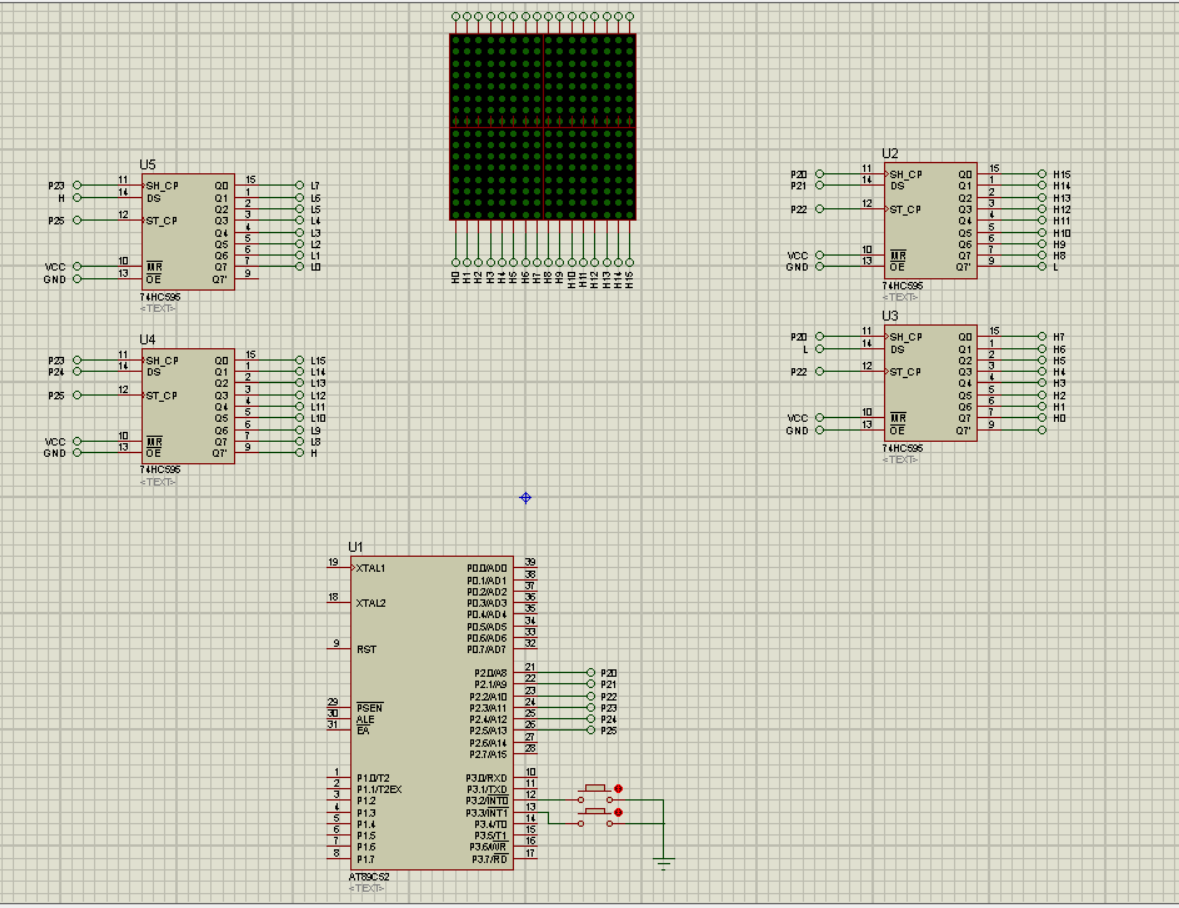
\includegraphics[scale=0.6]{billboard.png}
\end{figure}
\subsection{background music}
\begin{figure}[ht]
	\centering
	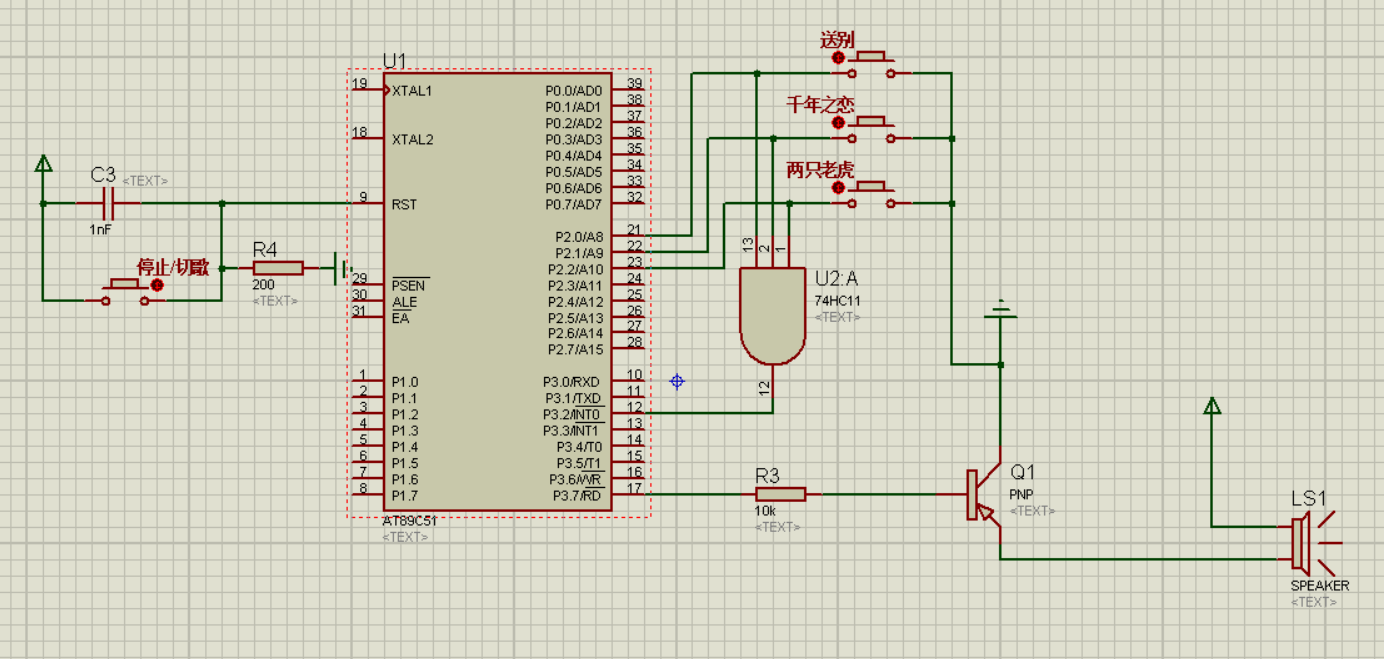
\includegraphics[scale=0.6]{backgroundmusic.png}
\end{figure}
\subsection{eating snake}
\begin{figure}[ht]
	\centering
	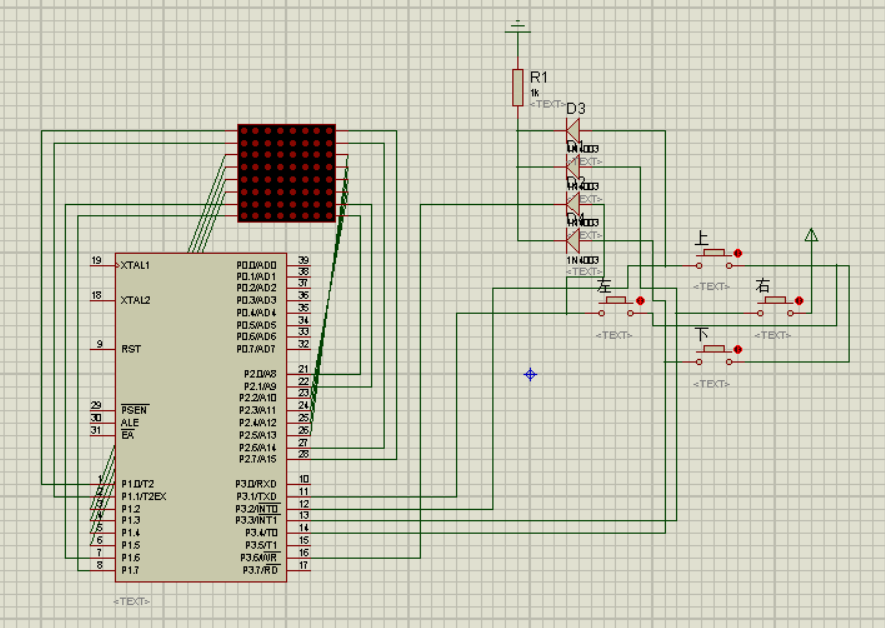
\includegraphics[scale=0.6]{snake.png}
\end{figure}
\end{document} 